%%%%%%%%%%%%%%%%%%%%%%%%%%%%%%%%%%%%%%%%%
% Short Sectioned Assignment
% LaTeX Template
% Version 1.0 (5/5/12)
%
% This template has been downloaded from:
% http://www.LaTeXTemplates.com
%
% Original author:
% Frits Wenneker (http://www.howtotex.com)
%
% License:
% CC BY-NC-SA 3.0 (http://creativecommons.org/licenses/by-nc-sa/3.0/)
%
%%%%%%%%%%%%%%%%%%%%%%%%%%%%%%%%%%%%%%%%%

%----------------------------------------------------------------------------------------
%	PACKAGES AND OTHER DOCUMENT CONFIGURATIONS
%----------------------------------------------------------------------------------------

\documentclass[paper=a4, fontsize=11pt]{scrartcl} % A4 paper and 11pt font size

\usepackage[T1]{fontenc} % Use 8-bit encoding that has 256 glyphs
\usepackage{fourier} % Use the Adobe Utopia font for the document - comment this line to return to the LaTeX default
\usepackage[english]{babel} % English language/hyphenation
\usepackage{amsmath,amsfonts,amsthm} % Math packages

\usepackage{minted} % Allows to put our code :)
\usepackage{graphicx} % Allows to put images :)
\usepackage[usenames, dvipsnames]{color} % Allows to have color :)

\usepackage{sectsty} % Allows customizing section commands
\allsectionsfont{\centering \normalfont\scshape} % Make all sections centered, the default font and small caps

\usepackage{fancyhdr} % Custom headers and footers
\pagestyle{fancyplain} % Makes all pages in the document conform to the custom headers and footers
\fancyhead{} % No page header - if you want one, create it in the same way as the footers below
\fancyfoot[L]{} % Empty left footer
\fancyfoot[C]{} % Empty center footer
\fancyfoot[R]{\thepage} % Page numbering for right footer
\renewcommand{\headrulewidth}{0pt} % Remove header underlines
\renewcommand{\footrulewidth}{0pt} % Remove footer underlines
\setlength{\headheight}{13.6pt} % Customize the height of the header

\numberwithin{equation}{section} % Number equations within sections (i.e. 1.1, 1.2, 2.1, 2.2 instead of 1, 2, 3, 4)
\numberwithin{figure}{section} % Number figures within sections (i.e. 1.1, 1.2, 2.1, 2.2 instead of 1, 2, 3, 4)
\numberwithin{table}{section} % Number tables within sections (i.e. 1.1, 1.2, 2.1, 2.2 instead of 1, 2, 3, 4)

\setlength\parindent{0pt} % Removes all indentation from paragraphs - comment this line for an assignment with lots of text

%----------------------------------------------------------------------------------------
%	TITLE SECTION
%----------------------------------------------------------------------------------------

\newcommand{\horrule}[1]{\rule{\linewidth}{#1}} % Create horizontal rule command with 1 argument of height

\title{
\normalfont \normalsize
\textit{In The Name of God} \\
\textsc{Computer Engineering Department of Amirkabir University of Technology} \\ [25pt]
\horrule{0.5pt} \\[0.4cm] % Thin top horizontal rule
\huge FPGA Homework - 6 \\ % The assignment title
\horrule{2pt} \\[0.5cm] % Thick bottom horizontal rule
}

\author{Parham Alvani (9231058)}

\date{\normalsize\today}

\begin{document}

\maketitle

%------- P1

\section{Problem 1}
\par Intellectual property core, IP core, or IP block is a reusable unit of
logic, cell, or chip layout design that is the intellectual property of one party.
\par We use IP cores in order to design our system modular.
\par IP cores must be:
\begin{itemize}
	\item
		understandable behavioural code of IP
	\item
		testability
	\item
		register output
	\item
		customizable and configurable
	\item
		proper number of I/O ports
\end{itemize}
\par USB interface, CORDIC, MD5, ...
\par IP cores categorize into following groups:
(flexibility and portability decrease from top to down)
\begin{itemize}
	\item
		Soft IP
	\item
		Firm IP
	\item
		Hard IP
\end{itemize}

%------- P2

\section{Problem 2}
\par FPGA special-purpose blocks like DSP,...

%------- P3

\section{Problem 3}
\par We use floorplaning for distributes design modules in FPGA, we assign
specific area of FPGA to design modules.

%------- P4

\section{Problem 4}
\par The critical path is defined as the path between an input and an output with the maximum delay.
\par The false path is defined as the path that never happend.
\par Some combinational paths from FF to another have more time than a one clock cycle.

%------- P5

\section{Problem 5}
\center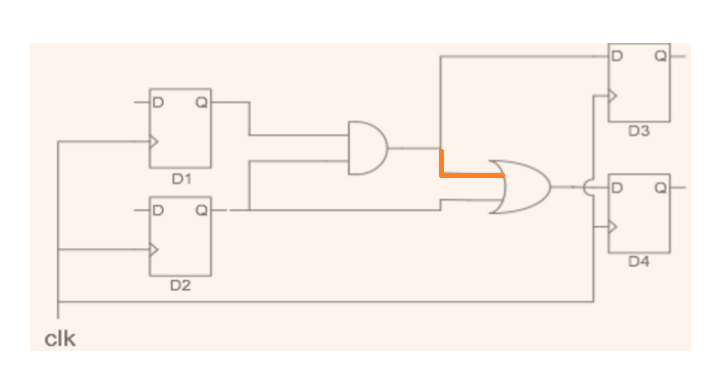
\includegraphics[]{p5-1.png}\\
\center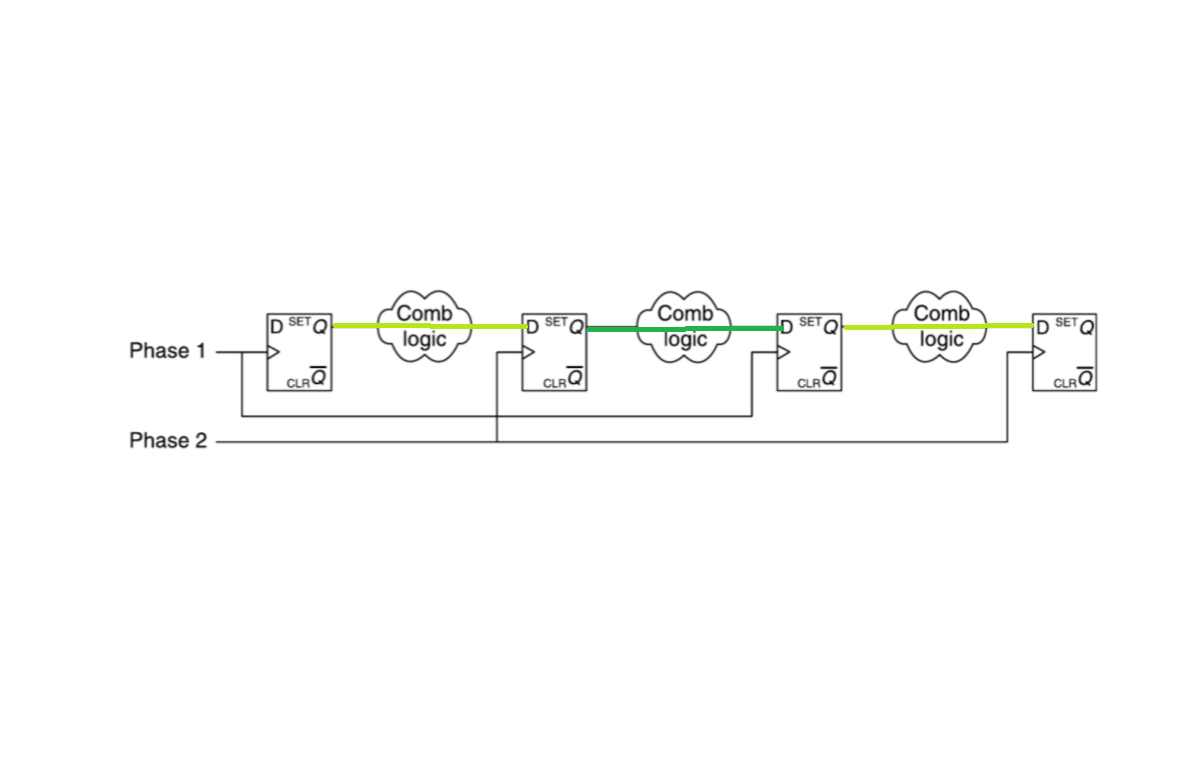
\includegraphics[]{p5-2.png}\\
\center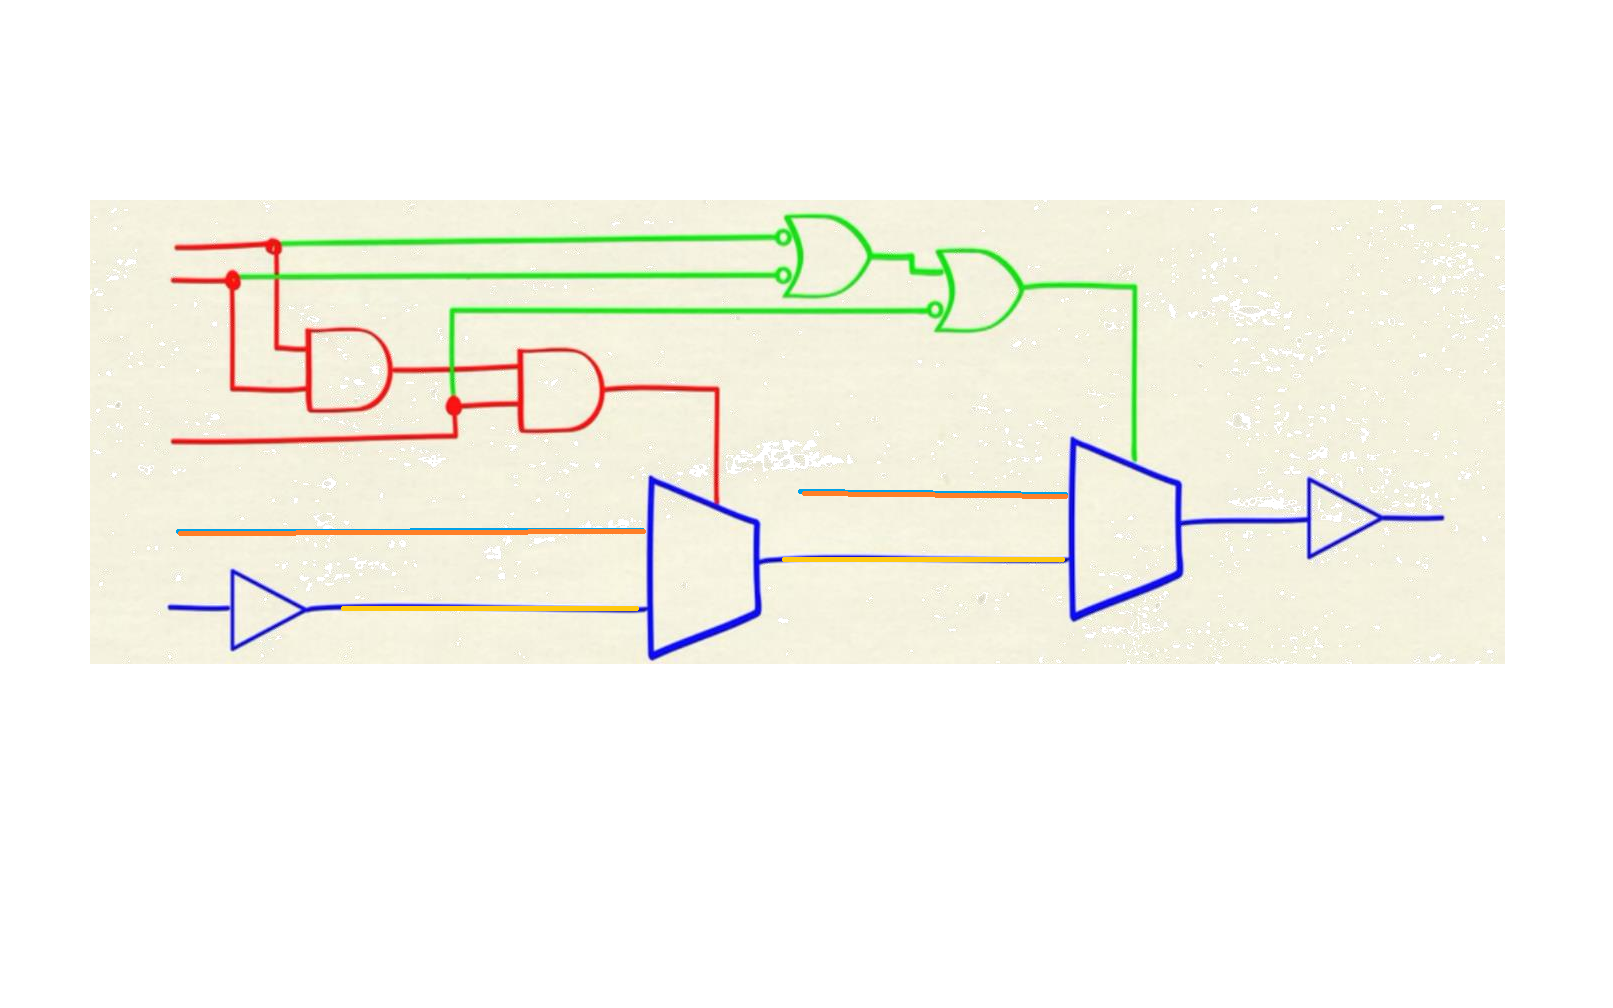
\includegraphics[]{p5-3.png}\\


%------- P6

\section{Problem 6}
\par 2 Full Adder (without resource sharing)
\inputminted{vhdl}{src/p6/p6-1.vhd}
\par 1 Full Adder (with resource sharing)
\inputminted{vhdl}{src/p6/p6-2.vhd}

%------- P7

\section{Problem 7}
\par
\begin{itemize}
	\item Memory Block Size: $1K * 10$
	\item Address: $X & Y$
\end{itemize}
\par
\begin{itemize}
	\item Memory Block Size: $4K * 2$
	\item Address: $X & Y$
\end{itemize}

%------- P8

\section{Problem 8}

\inputminted{vhdl}{src/p8/control.vhd}
\inputminted{vhdl}{src/p8/counter.vhd}
\inputminted{vhdl}{src/p8/datapath.vhd}
\inputminted{vhdl}{src/p8/main.vhd}
\inputminted{vhdl}{src/p8/main_t.vhd}

\end{document}
